\chapter{Solução proposta}
\section{Eletrônica}
\section{Energia}
\section{Estrutura}
\section{Software}
\subsection{Detalhamento dos softwares}
Radares usados no trânsito das cidades necessitam se comunicar com outros sistemas, tanto para passarem as informações obtidas dos automóveis monitorados quanto dados sobre o próprio funcionamento.

Além disso, é necessário às equipes que dão manutenção aos radares terem condições de obterem dados do funcionamento do sistema deles, para decidirem se e qual intervenção necessitarão fazer no equipamento.

Tendo isso em vista, serão criados 2 softwares para dar suporte ao funcionamento do radar: um serviço de monitoramento remoto dos radares e uma aplicação a ser usada por equipes de manutenção no diagnóstico dos equipamentos.

Abaixo está um diagrama que mostra como esses softwares interagirão com o radar:

\begin{figure}[!htb]
    \center{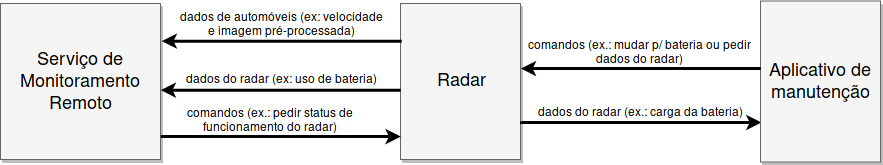
\includegraphics[width=\textwidth]{diagrama-in-out-software.png}}
    \caption{\label{fig:diagrama-in-out-software} Diagrama de inputs e outputs do radar e dos softwares}
\end{figure}

Nas sessões abaixo, serão melhor detalhados os softwares, assim como as funcionalidades deles.

\subsection{Serviço de Monitoramento Remoto (SMR)}

Este serviço, que é um dashboard que possui um servidor de microsserviços que dá suporte a ele, terá a função de obter os dados sobre automóveis enviados pelos radares, receber informações sobre o funcionamento dos equipamentos (por exemplo, se eles estão com a bateria ou os LEDs funcionando) e a partir disso realizar diversas operações.

As funcionalidades desse serviço serão:

\subsubsection{Recepção dos dados dos radares}

Os dados enviados por todos os radares serão recebidos pelo SMR e armazenados no banco de dados.

\subsubsection{Processamento de imagens de veículos}

As imagens enviadas pelos radares virão pré-processadas. Caberá ao SMR fazer o restante do processamento delas e, a partir disso, pegar as informações da placa dos automóveis.

\subsubsection{Verificação da placa do veículo}

O SMR irá checar todas as placas identificadas para saber se o automóvel fotografado foi furtado. Para isso, o SMR acessará o Sinesp ou outro serviço que permita consultar a situação do veículo.

\subsubsection{Notificação de irregularidades às autoridades}

Quando um radar fotografar um veículo furtado ou que ultrapassou a velocidade máxima permitida, o serviço irá mandar os dados do automóvel flagrado para as autoridades competentes, para que elas tomem as medidas cabíveis.

Alguns dos dados que serão enviados são a placa, o dia, o horário e a localização do radar que capturou o veículo.

\subsubsection{Notificação de possíveis acidentes}

Quando um radar enviar para o serviço uma notificação de possível acidente no local monitorado por ele, o SMR irá notificar uma central que, através de câmeras, irá confirmar se realmente houve um acidente. 

Caso não haja câmeras no local, o serviço irá notificar diretamente os bombeiros mais próximos da região onde fica o radar.

\subsubsection{Exibição de dados sobre os radares}

O serviço receberá dados sobre todos os equipamentos que se conectarem com ele, como status de funcionamento e problemas com algum componente. 

Essas informações poderão ser visualizadas ou usadas em análises de dados.

\subsubsection{Exibição de dados enviados pelos radares sobre veículos}

O serviço armazenará os dados sobre as informações relacionadas à veículos enviadas pelos radares, tais como quantidade de imagens enviadas e número de carros flagrados acima da velocidade permitida.

Essas informações poderão ser visualizadas ou usadas em análises de dados.

\subsection{Aplicativo de Manutenção}

Esse aplicativo mobile terá como principal objetivo auxiliar as pessoas responsáveis pela manutenção dos radares a diagnosticar como está o funcionamento deles.

As principais funcionalidades dele serão:

\subsubsection{Exibição de informações sobre o funcionamento do radar}

Através do aplicativo o responsável pela manutenção poderá saber como está o funcionamento de componentes do radar como, por exemplo, dos LEDs e da bateria.

\subsubsection{Alteração da fonte de energia do radar}

Através do aplicativo o responsável pela manutenção poderá mudar a fonte de alimentação do radar para a bateria ou para a fonte de energia externa.